\documentclass[12pt,class=report,crop=false]{standalone}
\usepackage[screen]{../python}

\pagestyle{empty}

\begin{document}


%====================================================================
\chapitre{Graphes et combinatoire de Ramsey}
%====================================================================


\begin{center}
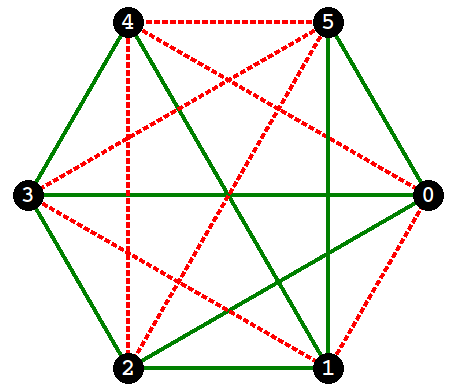
\includegraphics[scale=0.4]{ecran-ramsey-1d}
\end{center} 

\bigskip
\bigskip

\myfigure{0.8}{
  \tikzinput{fig-ramsey-0a}
}

\bigskip
\bigskip

\myfigure{0.4}{
  \tikzinput{fig-ramsey-0b}
}

\newpage

Voici un exemple de graphe à $5$ sommets qui possède $3$ sommets étrangers (les sommets $0$, $2$ et $4$), même s'il ne possède pas trois amis.

\myfigure{0.5}{
  \tikzinput{fig-ramsey-0c}
}

\bigskip
\bigskip

\mybox{\textbf{Proposition.} Dans un groupe de $6$ personnes, il y a toujours $3$ amis (les trois se connaissent deux à deux) ou $3$ étrangers (les trois sont tous des inconnus les uns pour les autres).}

\bigskip
\bigskip

\begin{center}
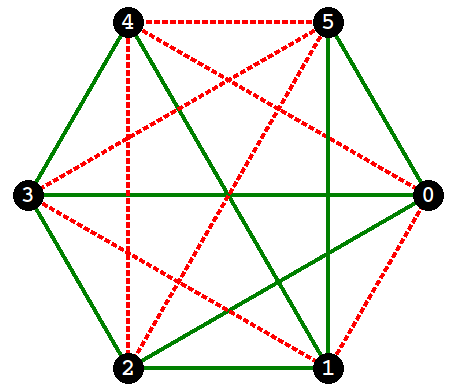
\includegraphics[scale=0.4]{ecran-ramsey-1d}
\end{center} 

\bigskip
\bigskip

  \begin{center}
  \begin{tabular}{|c|c|c|}
  \hline
  Nombre de sommets & Nombre de graphes & Temps de calcul approximatif \\
  \hline\hline
  $n=6$ & 32\,768 & $< 1$ seconde \\
  $n=7$ & 2\,097\,152 & $< 1$ minute \\  
  $n=8$ & 268\,435\,456 & $< 1$ heure \\
  $n=9$ & 68\,719\,476\,736 & $< 10$ jours \\ 
  \hline
  \end{tabular} 
  \end{center}
  
  
  
\newpage

\textbf{Modélisation}


\myfigure{0.7}{
  \tikzinput{fig-ramsey-1a}
}

\myfigure{0.7}{
  \tikzinput{fig-ramsey-1c}
}

\bigskip
\bigskip
\begin{center}

   \ci{graphe = [[0 for j in range(n)] for i in range(n)]}
\bigskip
\bigskip   
   
   \ci{graphe[i][j] = 1} \quad et \quad \ci{graphe[j][i] = 1}
\end{center}  
  
%  \item \ci{voir_graphe(graphe)}
%  
%\begin{center}
%\ci{00110}\\
%\ci{00101}\\
%\ci{11000}\\
%\ci{10001}\\
%\ci{01010}\\
%\end{center}
%
%  \item \ci{contient_3_amis_fixes(graphe,i,j,k)} 
%  \item \ci{contient_3_etrangers_fixes(graphe,i,j,k)} 
%\end{itemize}


  
\newpage

\textbf{Sous-ensembles}

Soit $E_n = \{0,1,2,\ldots,n-1\}$ l'ensemble des entiers de $0$ à $n-1$. L'ensemble $E_n$ contient donc $n$ éléments.

Par exemple $E_3 = \{ 0,1,2 \}$, $E_4 = \{ 0,1,2,3 \}$\ldots

\bigskip

\textbf{Exemple.}

Il y a $8$ sous-ensembles de $E_3$, ce sont :
    \begin{itemize}
      \item le sous-ensemble $\{0\}$ composé du seul élément $0$ ;
      \item le sous-ensemble $\{1\}$ composé du seul élément $1$ ;      
      \item le sous-ensemble $\{2\}$ composé du seul élément $2$ ; 
      \item le sous-ensemble $\{0,1\}$ composé de l'élément $0$ et de l'élément $1$ ;           
      \item le sous-ensemble $\{0,2\}$ ;
      \item le sous-ensemble $\{1,2\}$ ; 
      \item le sous-ensemble $\{0, 1,2\}$ composé de tous les éléments ;
      \item l'ensemble vide $\varnothing$ qui ne contient aucun élément !    
    \end{itemize} 

\medskip

\textbf{Proposition.} L'ensemble $E_n$ contient $2^n$ sous-ensembles.

\newpage

\textbf{Exemple.} $n = 6$ et $p=26$.
\begin{itemize}
  \item L'écriture binaire de $p=26$ sur $n=6$ \emph{bits} est 
  \ci[0,1,1,0,1,0],
  \item il y a des $1$ au rang $1$, $2$ et $4$ (en commençant au rang $0$ à gauche),
  \item le sous-ensemble associé est alors $\{1,2,4\}$.
\end{itemize}


\myfigure{0.7}{
  \tikzinput{fig-ramsey-4a}
}


\bigskip
\bigskip
\bigskip


\textbf{Exemple.} $n = 8$ et $p = 57$ 
\begin{itemize}
  \item L'écriture binaire sur $8$ \emph{bits} est \ci{[0,0,1,1,1,0,0,1]},
  \item le sous-ensemble associé correspond aux rangs $2,3,4,7$,
  \item c'est donc $\{2,3,4,7\}$.
\end{itemize}  

\myfigure{0.6}{
  \tikzinput{fig-ramsey-4b}
}  



\end{document}
